\chapter[Notes on Data Structuring]{Notes on Data Structuring\footnote{This monograph is based on a series of lectures delivered at a Nato Summer School, Marktoberdorf, 1970.}}

{
	\noindent
	\scshape\hfill\scriptsize C. A. R. HOARE\hfill
}
\renewcommand{\leftmark}{\normalfont\scriptsize\hfill C. A. R. HOARE\hfill}

\section{Introduction}

In the development of our understanding of complex phenomena, the most powerful tool available to the human intellect is abstraction. Abstraction arises from a recognition of similarities between certain objects, situations, or processes in the real world, and the decision to concentrate on these similarities, and to ignore for the time being the differences. As soon as we have discovered which similarities are relevant to the prediction and control of future events, we will tend to regard the similarities as fundamental and the differences as trivial. We may then be said to have developed an abstract concept to cover the set of objects or situations in question. At this stage, we will usually introduce a word or picture to symbolize the abstract concept; and any particular spoken or written occurrence of the word or picture may be used to \textit{represent} a particular or general instance of the corresponding situation.

The primary use for representations is to convey information about important aspects of the real world to others, and to record this information in written form, partly as an aid to memory and partly to pass it on to future generations. However, in primitive societies the representations were sometimes believed to be useful in their own right, because it was supposed that manipulation of representations might in itself cause corresponding changes in the real world; and thus we hear of such practices as sticking pins into wax models of enemies in order to cause pain to the corresponding part of the real person. This type of activity is characteristic of magic and witchcraft. The modern scientist on the other hand, believes that the manipulation of representations could be used to predict events and the results of changes in the real world, although not to cause them. For example, by manipulation of symbolic representations of certain functions and equations, he can predict the speed at which a falling object will hit the ground, although he knows that this will not either cause it to fall, or soften the final impact when it does.

The last stage in the process of abstraction is very much more sophisticated; it is the attempt to summarize the most general facts about situations and objects covered under an abstraction by means of brief but powerful \textit{axioms}, and to prove rigorously (on condition that these axioms correctly describe the real world) that the results obtained by manipulation of representations can also successfully be applied to the real world. Thus the axioms of Euclidean geometry correspond sufficiently closely to the real and measurable world to justify the application of geometrical constructions and theorems to the practical business of land measurement and surveying the surface of the earth.

The process of abstraction may thus be summarized in four stages:

\begin{enumerate}[leftmargin=2\parindent, label=(\arabic*)]
	\item Abstraction: the decision to concentrate on properties which are shared  by many objects or situations in the real world, and to ignore the differences between them.
	\item Representation: the choice of a set of symbols to stand for the abstraction; this may be used as a means of communication.
	\item Manipulation: the rules for transformation of the symbolic representations as a means of predicting the effect of similar manipulation of the real world.
	\item Axiomatization: the rigorous statement of those properties which have been abstracted from the real world, and which are shared by manipulations of the real world and of the symbols which represent it.
\end{enumerate}

\subsection{Numbers and Numerals}
Let us illustrate this rather abstract description by means of a relatively concrete example --- the number four. In the real world, it is noticed that objects can be grouped together in collections, for example four apples. This already requires a certain act of abstraction, that is a decision to ignore (for the time being) the differences between the individual apples in the collection --- for example, one of them is bad, two of them unripe, and the fourth already partly eaten by birds.

Now one may consider several different collections, each of them with four items; for example, four oranges, four pears, four bananas, etc. If we choose to ignore the differences between these collections and concentrate on their similarity, then we can form a relatively abstract concept of the number four. The same process could lead to the concept of the number 3, 15, and so on; and a yet further stage of abstraction would lead to the development of the concept of a natural number.

Now we come to the representation of this concept, for example scratched on parchment, or carved in stone. The representation of a number is called a numeral. The early Roman numeral was clearly pictorial, just four strokes carved in stone: IIII. An alternative more convenient representation was IV. The arabic (decimal) representations are less pictorial, but again there is some choice: both 4 and 04 (and indeed 004 and so on) are all recognized as valid numerals, representing the same number.

We come next to a representation which is extremely convenient for processing, providing that the processor is an electronic digital computer. Here the number four is represented by the varying directions of magnetization of a group of ferrite cores. These magnetization are sometimes represented by sequences of zeros and ones on line printer paper; i.e., the binary representation of the number in question.

A simple example of the manipulation of numerals is addition, which can be used to predict the result of adjoining of two collections of objects in the real world. The addition rules for Roman numerals are very simple and obvious, and are simple to apply. The addition rules for arabic numerals up to ten are quite unobvious, and must be learnt; but for numbers much larger than ten they are more convenient than the Roman techniques. Addition of binary representations is not a task fit for human beings; but for a computer this is the simplest and best representation. Thus we see that choice between many representations can be made in the light of ease of manipulation in each particular environment.

Finally we reach the stage of axiomatization; the most widely known axiom set for natural numbers is that of Peano, which was first formulated at the end of the last century, long after natural numbers had been in general use. In the present day, the axiomatization of abstract mathematical ideas usually follows far more closely upon their development; and in fact may assist in the clarification of the concept by guarding against confusion and error, and by explaining the essential features of the concept to others. It is possible that a rigorous formulation of presuppositions and axioms on which a program is based may reduce the confusion and error so characteristic of present day programming practice, and assist in the documentation and explanation of programs and programming concepts to others.

\subsection{Abstraction and computer programming}

It is my belief that the process of abstraction, which underlies attempts to apply mathematics to the real world, is exactly the process which underlies the application of computers in the real world. The first requirement in designing a program is to concentrate on relevant features of the situation, and to ignore factors which are believed irrelevant. For example, in analyzing the flutter characteristics of a proposed wing design of an aircraft, its elasticity is what is considered relevant; its color, shape, and production technique are considered to be irrelevant except in so far as they have contributed to its elasticity. To take a commercial example, the employees working for a Company have many characteristics, both physical and mental, which will be ignored when devising a payroll program for the Company.

The next stage in program design is the decision of the manner in which the abstracted information is to be represented in the computer. An elasticity function may be represented by its values at a suitable number of discrete points; and these may be represented in a variety of ways as a two-dimensional array. Alternatively, the elasticity might be given by a computed function, and the data be held as a vector of polynomial or chebyshev coefficients for the function. A payroll file on a computer consists of a number of records, one relating to each employee. The choice of representation within the record of each relevant attribute must be made as part of the design of the program.

The stage of axiomatization is not usually regarded as a separate stage in programming; and is often left implicit. In the case of aircraft flutter, the axiomatization is the formulation of the differential equations which are presumed to describe the reaction of the real wing to certain kinds of stresses, and which (it is hoped) also describe the process of approximate solution on the computer. In the case of a payroll, the axioms correspond to the descriptions of various aspects of the real world which need to be embodied in the program --- for example, the fact that net pay equals gross pay minus deductions.

Finally there comes the task of programming the computer to get it to carry out those manipulations on the representation of the data that correspond to the manipulations in the real world in which we are interested. 

The success of a program is dependent on three basic conditions:

\begin{enumerate}[leftmargin=2\parindent, label=(\arabic*)]
	\item The axiomatisation is a correct description of those aspects of the real world with which it is concerned.
	\item The axiomatisation is a correct description of the behavior of the program, i.e., that the program contains no errors.
	\item The choice of representation and the method of manipulation are such that the cost of running the program on the computer is acceptable.
\end{enumerate}

In order to simplify the task of designing and developing a computer program, it is very helpful to be able to keep these three stages reasonably separate and to carry them out in the appropriate sequence. Thus the first stage (axiomatisation) would culminate in a rigorous logical statement of presuppositions about the real world, and a formulation of the desired objectives which are to be achieved by the program. The second stage would culminate in an algorithm, or abstract program, which is demonstrably capable of carrying out the stated task on the given presuppositions. The third stage would be the decision on how the various items of data are to be represented and manipulated in the store of the computer in order to achieve acceptable efficiency. Only when these three stages have been satisfactorily concluded will there begin the final phase of coding and testing the program, which embodies the chosen algorithm operating upon the chosen data representation.

Of course, this is a somewhat idealized picture of the intellectual task of programming as a steady progression from the abstract formulation of the problem to the more and more concrete aspects of its solution. In practice, even in the formulation of a problem, the programmer must have some intuition about the possibility of a solution; while he is designing his abstract program, he must have some feeling that an adequately efficient representation is available. Quite frequently these intuitions and feelings will be mistaken,
and a deeper investigation of representation, or even the final coding, will require a return to an earlier stage in the process, and perhaps even a radical recasting of the direction of attack. But this exercise of intuitive forethought, together with a risk of failure, is characteristic of all inventive and constructive intellectual processes, and does not detract from the merits of at least starting out in an orderly fashion, with more or less clearly separated stages.

One of the most important features of the progression is that the actual coding of the program has been postponed until after it is (almost) certain that all other aspects of the design have been successfully completed. Since coding and program testing is generally the most expensive stage in program development, it is undesirable to have to make changes after this stage has started. Thus it is advantageous to ensure beforehand that nothing further can go wrong at this final stage; for example, that the program tackles the right problem, that the algorithm is correct, that the various parts of the program cooperate harmoniously in the overall task, and that the data representations are adequately efficient. It is the purpose of this monograph to explore methods of achieving this confidence.

\subsection{Abstraction in high-level programming languages}

The role of abstraction in the design and development of computer programs may be reinforced by the use of a suitable high-level programming language. Indeed, the benefits of using a high-level language instead of machine code may be largely due to their incorporation of successful abstractions, particularly for data. To the hardware of a computer, and to a machine code programmer, every item of data is regarded as a mere collection of bits. However, to the programmer in ALGOL 60 or FORTRAN an item of data is regarded as an integer, a real number, a vector, or a matrix, which are the same abstractions that underlie the numerical application areas for which these languages were primarily designed. Of course, these abstract concepts have been mapped by the implementer of the language onto particular bit-pattern representations on a particular computer. But in the design of his algorithm, the programmer is freed from concern about such details, which for his purpose are largely irrelevant; and his task is thereby considerably simplified.

Another major advantage of the use of high-level programming languages, namely machine-independence, is also attributable to the success of their abstractions. Abstraction can be applied to express the important characteristics not only of differing real-life situations, but also of different computer representations of them. As a result, each implementer can select a representation which ensures maximum efficiency of manipulation on his particular computer.

A third major advantage of the use of a high-level language is that it significantly reduces the scope for programming error. In machine code programming it is all too easy to make stupid mistakes, such as using fixed point addition on floating point numbers, performing arithmetic operations on Boolean markers, or allowing modified addresses to go out of range. When using a high-level language, such errors may be prevented by three means:

\begin{enumerate}[leftmargin=2\parindent, label=(\arabic*)]
	\item Errors involving the use of the wrong arithmetic instructions are logically impossible; no program expressed, for example in ALGOL, could ever cause such erroneous code to be generated.
	\item Errors like performing arithmetic operations on Boolean markers will be immediately detected by a compiler, and can never cause trouble in an executable program.
	\item Errors like the use of a subscript out of range can be detected by runtime checks on the ranges of array subscripts.
\end{enumerate}

Runtime checks, although often necessary, are almost unavoidably more expensive and less convenient than checks of the previous two kinds; and high-level languages should be designed to extend the range of programming errors which logically cannot be made, or if made can be detected by a compiler. In fact, skillful language design can enable most subscripts to be checked without loss of runtime efficiency.

The automatic prevention and detection of programming errors may again be attributed to a successful appeal to abstraction. A high-level programming language permits the programmer to declare his intentions about the types of the values of the variables he uses, and thereby specify the meanings of the operations valid for values of that type. It is now relatively easy for a compiler to check the consistency of the program, and prevent errors from reaching the execution stage.

\subsection{Notations}

In presenting a theory of data structuring, it is necessary to introduce some convenient notation for expressing the abstractions involved. These notations are based to a large extent on those already familiar to mathematicians, logicians and programmers. They have also been designed for direct expression of computer algorithms, and to minimize the scope for programming error in running programs. Finally, the notations are designed to ensure the existence of efficient data representations on digital computers. Since the notations are intended to be used (among other things) for the expression of algorithms, it would be natural to conclude that they constitute a form of programming language, and that an automatic translator should be written for converting programs expressed in the language into the machine code of a computer, thereby eliminating the expensive and error-prone coding stage in the development of programs.

But this conclusion would be a complete misunderstanding of the reason for introducing the notations, and could have some very undesirable consequences. The worst of them is that it could lead to the rejection of the main benefits of the programming methodology expounded in this monograph, on the grounds that no compiler is available for the language, nor likely to be widely accepted if it were.

But there are sound reasons why these notations must not be regarded as a programming language. Some of the operations (e.g., concatenation of sequences), although very helpful in the design of abstract programs and the description of their properties, are grotesquely inefficient when applied to large data objects in a computer; and it is an essential part of the program design process to eliminate such operations in the transition between an abstract and a concrete program. This elimination will sometimes involve quite radical changes to both algorithm and representation, and could not in general be made by an automatic translator. If such expensive operators were part of a language intended for automatic compilation, it is probable that many programmers would fail to realize their obligation to eliminate them before approaching the computer; and even if they wanted to, they would have little feeling for what alternative representations and operations would be more economic. In taking such vital decisions, it is actually helpful if a programming language is rather close to the eventual machine, in the sense that the efficiency of the machine code is directly predictable from the form and length of the corresponding source language code.

There is a more subtle danger which would be involved in the automatic implementation of the notations: that the good programmer would soon learn that some of them are significantly less efficient than others, and he will avoid their use even in his abstract programs; and this will result in a form of mental block which might have serious consequences on his inventive capacity. Equally serious, the implementation of a fixed set of notations might well inhibit the user from introducing his own notations and concepts as required by his understanding of a particular problem.

Thus there is a most important distinction to be drawn between an algorithmic language intended to assist in the definition, design, development and documentation of a program, and the programming language in which the program is eventually conveyed to a computer. In this monograph we shall be concerned solely with the former kind of language. All example algorithms will be expressed in this language, and the actual coding of these programs is left as an exercise to the reader, who may choose for this purpose any language familiar to him, ALGOL, FORTRAN, COBOL, PL/I, assembly language, or any available combination of them. It is essential to a realization of the relative merits of various representations of data to realize what their implications on the resulting code will be.

In spite of this vigorous disclaimer that I am not embarking on the design of yet another programming language, I must admit the advantages that can follow if the programming language used for coding an algorithm is actually a \textit{subset} of the language in which it has been designed. I must also confess that there exists a large subset of the proposed algorithmic language which can be implemented with extremely high efficiency, both at compile time and at run time, on standard computers of the present day; and the challenge of designing computers which can efficiently implement even larger subsets may be taken up in the future. But the non-availability of such a subset implementation in no way invalidates the benefits of using the full set of notations as an abstract programming tool.

\subsection{Summary}

This introduction has given a general description of the motivation and general approach taken hereafter. As is quite usual, it may be read again with more profit on completion of the rest of the monograph.

The second section explains the concept of type, which is essential to the theory of data structuring; and relates it to the operations and representations which are relevant to the practice of computer programming.

Subsequent sections deal with particular methods of structuring data, progressing from the simpler to the more elaborate structures.

Each structure is explained informally with the aid of examples. Then the manipulation of the structure is defined by specifying the set of basic operations which may be validly applied to the structure. Finally, a range of possible computer representations is given, together with the criteria which should influence the selection of a suitable representation on each occasion.

Section 11 is devoted to an example, a program for constructing an examination timetable. The last section puts the whole exposition on a rigorous theoretical basis by formulating the axioms which express the basic properties of data structures. This section may be used as a summary of the theory, as a reference to refine the understanding, or as a basis for the proof of correctness of programs.

\section{The concept of type}

The theory of data structuring here propounded is strongly dependent on the concept of type. This concept is familiar to mathematicians, logicians, and programmers.

(1) In mathematical reasoning, it is customary to make a rather sharp distinction between individuals, sets of individuals, families of sets, and so on; to distinguish between real functions, complex functions, functionals, sets off unctions, etc. In fact for each new variable introduced in his reasoning, a mathematician usually states immediately what type of object the variable can stand for, e.g.

\quad ``Let $f$ be a real function of two real variables''

\quad ``Let $S$ be a family of sets of integers''.

Sometimes in mathematical texts a general rule is given which relates the type of a symbol with a particular printer's type font, for example:

\hangindent=1.9\parindent \quad``We use small Roman letters to stand for individuals, capitals to stand for sets of individuals, and script capitals to denote families of sets''.

In general, mathematicians do not use type conventions of this sort to make distinctions of an arbitrary kind; for example, they would not be generally used to distinguish prime numbers from non-primes or Abelian groups from general groups. In practice, the type conventions adopted by mathematicians are very similar to those which would be of interest to logicians and programmers.

(2) Logicians on the whole prefer to work without typed variables. However without types it is possible to formulate within set theory certain paradoxes which would lead to inescapable contradiction and collapse of logical and mathematical reasoning. The most famous of these is the Russell paradox:

\quad \hspace{-.4em}``let $s$ be the set of all sets which are \textit{not} members of themselves.

\quad Is $s$ a member of itself or not?''

\noindent
It turns out that whether you answer yes or no, you can be immediately proved wrong.

Russell's solution to the paradox is to associate with each logical or mathematical variable a \textit{type}, which defines whether it is an individual, a set, a set of sets, etc. Then he states that any proposition of the form ``$x$ is a member of $y$'' is grammatically meaningful only if $x$ is a variable of type individual and $y$ a variable of type set, or if $x$ is of type set and $y$ is of type set of sets, and so on. Any proposition that violates this rule is regarded as meaningless --- the question of its truth or falsity just does not arise, it is just a jumble of letters. Thus any proposition involving sets that are or are not members of themselves can simply be ruled out.

Russell's theory of types leads to certain complexities in the foundation of mathematics, which are not relevant to describe here. Its interesting features for our purposes are that types are used to prevent certain erroneous expressions from being used in logical and mathematical formulae; and that a check against violation of type constraints can be made merely by scanning the text, without any knowledge of the value which a particular symbol might happen to stand for.

(3) In a high-level programming language the concept of a type is of central importance. Again, each variable, constant and expression has a unique type associated with it. In ALGOL 60 the association of a type with a variable is made by its declaration; in FORTRAN it is deduced from the initial letter of the variable. In the implementation of the language, the type information determines the representation of the values of the variable, and the amount of computer storage which must be allocated to it. Type information also determines the manner in which arithmetic operators are to be interpreted; and enables a compiler to reject as meaningless those programs which invoke inappropriate operations.

Thus there is a high degree of commonality in the use of the concept of type by mathematicians, logicians and programmers. The salient characteristics of the concept of type may be summarized:

\begin{enumerate}[leftmargin=2\parindent, label=(\arabic*)]
	\item A type determines the class of values which may be assumed by a variable or expression.
	\item Every value belongs to one and only one type.
	\item The type of a value denoted by any constant, variable, or expression may be deduced from its form or context, without any knowledge of its value as computed at run time.
	\item Each operator expects operands of some fixed type, and delivers a result of some fixed type (usually the same). Where the same symbol is applied to several different types (e.g. $+$ for addition of integers as well as reals), this symbol may be regarded as ambiguous, denoting several different actual operators. The resolution of such systematic ambiguity can always be made 	at compile time.
	\item  The properties of the values of a type and of the primitive operations defined over them are specified by means of a set of axioms.
	\item Type information is used in a high-level language both to prevent or detect meaningless constructions in a program, and to determine the method of representing and manipulating data on a computer.
	\item The types in which we are interested are those already familiar to mathematicians; namely, Cartesian Products, Discriminated Unions, Sets, Functions, Sequences, and Recursive Structures.
\end{enumerate}

\subsection{Data type definitions}

Our theory of data structuring specifies a number of standard methods of defining types, and of using them in the declaration of variables to specify the range of values which that variable may take in the course of execution of a program. In most cases, a new type is defined in terms of previously defined \textit{constituent} types; the values of such a new type are data structures, which can be built up from \textit{component} values of the constituent types, and from which the component values can subsequently be extracted. These component values will belong to the constituent types in terms of which the structured type was defined. If there is only one constituent type, it is known as the \textit{base} type.

The number of different values of a data type is known as its \textit{cardinality}. In many cases the cardinality of a type is finite; and for a structured type defined in terms of finite constituent types, the cardinality is also usually finite, and can be computed by a simple formula. In other cases, the cardinality of a data type is infinite, as in the case of integers; but it can never be more than denumerably infinite. The reason for this is that each value of the type must be constructible by a finite number of computer operations, and must be representable in a finite amount of store. Arbitrary real numbers, functions with infinite domains. and other classes of non-denumerable cardinality can never be represented as stored data within a computer, though in some cases they can be represented by procedures, functions, or other program structures.

Obviously, the ultimate components of a structure must be unstructured, and the ultimate constituents of a structured type must be unstructured types. One method of defining an unstructured type is by simple enumeration of its values, as described in the next section. But in certain cases it is better to regard the properties of unstructured types as defined by axioms, and assume them to be provided as \textit{primitive} types by the hardware of a computer or the implementation of a high-level programming language. For example, the primitive types of ALGOL 60 are \textbf{integer}, \textbf{real}, and \textbf{Boolean}, and these will be assumed available.

\subsection{Data manipulation}

The most important practical aspect of data is the manner in which that data can be manipulated, and the range of basic operators available for this purpose. We therefore associate with each type a set of \textit{basic} operators which are intended to be useful in the design of programs, and yet which have at least one reasonably efficient implementation on a computer. Of course the selection of basic operators is to some extent arbitrary, and could have been either larger or smaller. The guiding principle has been to choose a set large enough to ensure that any additional operation required by the programmer can be defined in terms of the basic set, and be efficiently implemented in this way also; so an operator is regarded as basic if its method of efficient implementation depends heavily on the chosen method of data representation.

The most important and general operations defined for data of any type are assignment and test of equality. Assignment involves conceptually a complete copy of a data value from one place to another in the store of the computer; and test of equality involves a complete scan of two values (usually stored at different places) to test their identity. These rules are those that apply to primitive data types and there is no reason to depart from them in the case of structured types. If the value of a structured type is very large, these operations may take a considerable amount of time; this can sometimes be reduced by an appropriate choice of representation; alternatively, such operations can be avoided or removed in the process of transforming an abstract program to a concrete one.

Another general class of operators consists in the \textit{transfer} functions, which map values of one type into another. Of particular importance are the \textit{constructors}, which permit the value of a structured type to be defined in terms of the values of the constituent types from which it is built. The converse transfer functions are known as \textit{selectors}; they permit access to the component values of a structured type. In many cases, we use the name of a defined type as the name of the standard constructor or transfer function which ranges over the type.

Certain data types are conveniently regarded as ordered; and comparison operators are available to test the values of such types. But for many types, such an ordering would have no meaningful interpretation; and such types are best regarded from an abstract point of view as unordered. This will sometimes be of advantage in giving greater freedom in the choice of representation and sequencing strategies at a later state in the concrete design.

In the case of a large data structure, the standard method of operating efficiently on it is not by assigning a wholly new value to it, but rather by \textit{selectively updating} some relatively small part of it. The usual notation for this is to write on the left of an assignment an expression (variable) which uses selectors to denote the place where the structure is to be changed. However, we also introduce special assignment operators, always beginning with colon, to denote other more general updating operations such as adding a member to a set, or appending an item to a sequence. For both kinds of selective updating, it must be remembered that, from a conceptual or abstract point of view, the entire value of the variable has been changed by updating the least part of it.

\subsection{Representations}

It is fundamental to the design of a program to decide how far to store computed results as data for subsequent use, and how far to compute them as required. It is equally fundamental to decide how stored data should be represented in the computer. In many simple and relatively small cases there is an obvious \textit{standard} way of representing data, which ensures that not too much storage is used, and not too much time expended on carrying out the basic operations. But if the volume of data (or the amount of processing) is large, it is often profitable (and sometimes necessary) to choose some non-standard representation, selected in accordance with the characteristics of the storage media used (drums, discs, or tapes), and also taking into account the relative frequencies of the various operations which will be performed upon it. Decisions on the details of representation must usually precede and influence the design of the code to manipulate the data, often at a time when the nature of the data and the processing required are relatively unknown. Thus it is quite common to make serious errors of judgment in the design of data representation, which do not come to light until shortly before, or even after, the program has been put into operation. By this time the error is extremely difficult to rectify. However, the use of abstraction in data structuring may help to postpone some of the decisions on data representation until more is known about the behavior of the program and the characteristics of the data, and thus make such errors less frequent and easier to rectify.

An important decision to be taken is on the degree and manner in which data should be compressed in storage to save space; and also to save time on input$/$output, on copying operations, and on comparisons, usually at the expense of increasing the time and amount of code required to perform all other operations. Representations requiring less storage than the standard are usually known as \textit{packed}; there are several degrees of packing, from loose to tight. Of theoretical interest is the \textit{minimal} representation, which uses the least possible space. In this representation the values of the type are represented as binary integers in the range 0 to $N - 1$, where $N$ is the cardinality of the type. In the case of a type of infinite cardinality, a minimal representation is one in which every possible bit pattern represents a value of the type. Minimal representations are not often used, owing to the great expense of processing them.

Another method of saving space is to use an \textit{indirect} representation. In the standard direct representation of data, each variable of a type is allocated enough space to hold every value of the type. In the indirect representation, the variable is just large enough to contain a single machine address, which at any given time points to a group of one or more machine locations containing the current value. This technique is necessary when the type has infinite cardinality, since the amount of storage used will vary, and is not known when writing the code which accesses the variable. It can also be profitable when the actual amount of storage is variable, and during a large part of a program run is significantly less than the maximum. Finally, it can be used when it is believed that many different variables will tend to have the same values; since then only one copy of the value need be held, and the variables may just contain pointers to it; copying the value is also very cheap, since only the pointer need be copied. However, such shared copies must never be selectively updated.

Unfortunately, indirect representations often involve the additional expense and complexity of a dynamic storage allocation and garbage collection scheme; and they can cause some serious problems if data has to be copied between main and backing stores.

This chapter describes only a small but useful range of the possible representations of data, and the skillful programmer could readily add to the selection. In many cases, the representation of an abstract data type can be constructed by means of a more elaborate but more efficient data type definition; for instance a large set may be represented as a sequence of items of some suitable type. Examples of this are given in later sections.

\section{Unstructured data types}

All structured data must in the last analysis be built up from unstructured components, belonging to a primitive or unstructured type. Some of these unstructured types (for example, reals and integers) may be taken as given by a programming language or the hardware of the computer. Although these primitive types are theoretically adequate for all purposes, there are strong practical reasons for encouraging a programmer to define his own unstructured types, both to clarify his intentions about the potential range of values of a variable, and the interpretation of each such value; and to permit subsequent design of an efficient representation.

In particular, in many computer programs an integer is used to stand not for a numeric quantity, but for a particular choice from a relatively small number of alternatives. In such cases, the annotation of the program usually lists all the possible alternative values, and gives the intended interpretation of each of them. It is possible to regard such a quantity as belonging to a separate type, quite distinct from the integer type, and quite distinct from any other similar set of markers which have a different interpretation. Such a type is said to be an \textit{enumeration}, and we suggest a standard notation for declaring the name of the type and associating a name with each of its alternative values:
\medskip

\tabto{3.7em}\textbf{type} suit $=$ (club, diamond, heart, spade);

\noindent
\hangindent=5.6\parindent\textbf{ordered} \tabto{3.7em}\textbf{type} rank = (two, three, four, five, six, seven, eight, nine, ten, Jack, Queen, King, Ace);
\medskip

\tabto{3.7em}\textbf{type} primary color $=$ (red, yellow, blue);

\noindent
\hangindent=7.4\parindent\textbf{ordered} \tabto{3.7em}\textbf{type} day of week $=$ (Monday, Tuesday, Wednesday, Thursday, Friday, Saturday, Sunday);
\medskip

\tabto{3.7em}\textbf{type} day of month $= 1\,.\,.\,31$;

\noindent
\hangindent=6.2\parindent\textbf{ordered} \tabto{3.7em}\textbf{type} month $=$ (Jan, Feb, March, April, May, June, July, Aug, Sept, Oct, Nov, Dec);
\medskip

\tabto{3.7em}\textbf{type} year $= 1900\,.\,.\,1969$;

\tabto{3.7em}\textbf{type} Boolean $=$ (false, true);
\medskip

\noindent
\hangindent=5.6\parindent\textbf{ordered} \tabto{3.7em}\textbf{type} floor $=$ (basement, ground, mezzanine, first, second);

\tabto{3.7em}\textbf{type} coordinate $= 0\,.\,.\,1023$;
\medskip

Our first two examples are drawn from the realm of playing cards. The first declaration states that club, diamond, heart, and spade are suits; in other words, that any variable or expression of type suit can only denote one of these four values; and that the identifiers ``club'' ``heart'' ``diamond'' and ``spade'' act as \textit{constants} of this type. Similarly, the definition of the type \textit{rank} displays the thirteen constants denoting the thirteen possible values of the type. In this case it is natural to regard the type as ordered. The next examples declare the names of the primary colors and of the days of the week. In considering the days of the month, it is inconvenient to write out the thirty-one possible values in full. We therefore introduce the convention that $a\,.\,.\,b$ stands for the finite range of values between $a$ and $b$ inclusive. This is known as a \textit{subrange} of the type to which $a$ and $b$ belong, in this case integers. This convention is used again in the declaration of year. Other examples of enumeration are:

\quad The Boolean type, with only two values, false and true.

\quad The Month type, with twelve values listed in the required order.

\hangindent=2.8\parindent\quad The coordinate type, taking values between 0 and 1023, representing perhaps a coordinate on a CRT display.

Having defined a type in a suitable fashion, the programmer will use the type name to specify the types of his variables. For this purpose it is useful to follow the current practice of mathematicians and to write the type name \textit{after} the variable, separated from it by a colon:

\quad trumps: suit; today:day of week;

\quad $pc$: primary color;

\noindent
If several variables of the same type are to be declared at the same time, it is useful to adopt the abbreviation of listing the variable names without repeating the type name, thus:

\quad arrival, departure: day of month;

\quad $x$, $y$, $z$: coordinate.

\noindent
If only a few variables of a given type are to be used, it is convenient to write the type definition itself in place of and instead of the type name:

\quad answer: (yes, no, don't know);

The cardinality of a type defined by enumeration is obviously equal to the length of the defining list; and for a numeric subrange, it is one more than the difference between the end points of the subrange.

\subsection{Manipulation}

The operations required for successful manipulation of values of enumeration types and subranges are:

\begin{enumerate}[leftmargin=2\parindent, label=(\arabic*)]
	\item test of equality, for example:

	\quad \textbf{if} arrival $=$ departure \textbf{then go} to transit desk;

	\quad \textbf{if} trumps $=$ spade \textbf{then} \dots

	\item assignment, for example·

	\quad $pc \coloneq$ yellow;

	\quad trumps $\coloneq$ club;

	\item \label{en:manipulation-3}
	case discrimination, for example:

	\quad \textbf{case} $p$c \textbf{of} (red: \dots,

	\tabto{5.7em}yellow: \dots,

	\tabto{5.7em}blue: \dots)
	
	where $pc$ is a variable or expression of type primary color, and the limbs of the discrimination are indicated by lacunae. A case discrimination may be either a statement, in which case the limbs must be statements; or it may be an expression, in which case the limbs must be all expressions of the same type.
	
	The effect of a case discrimination is to select for execution (or evaluation) that single statement (or expression) which is prefixed by the constant equal to the current value of the case expression. In some cases, it may be convenient to prefix several constants to the same limb, or even to indicate a subrange of values which would select the corresponding limb; but of course each value must be mentioned exactly once:
	
	\quad \textbf{case} digit \textbf{of} ($0\,.\,.\,2:\dots$,
	
	\tabto{6.6em}$3:7:\dots$,
	
	\tabto{6.6em}$4\,.\,.\,6:8:9:\dots$).
	
	\noindent
	In this last case, it would be convenient to replace the labels of the last limb by the basic word \textbf{else}, to cover all the remaining cases not mentioned explicitly on the preceding limbs.
	
	When the limbs of a discrimination are statements, we shall sometimes use braces instead of brackets to surround them.
	
	\item In the case of a type declared as ordered, it is possible to test the ordering relationships among the values:
	
	\quad \textbf{if} May $\leqslant$ this month \& this month $\leqslant$ September \textbf{then}
	
	\qquad adopt summer timetables. 
	
	\noindent
	In other cases, the ordering of the values is quite irrelevant, and has no meaning to the programmer.
	
	\item In conjunction with ordering, it is useful to introduce a successor and a predecessor function (succ and pred) to map each value of the type onto the next higher or lower value, if there is one. Also, if $T$ is any ordered type, the notation $T$.min will denote the lowest value of the type, and $T$.max the highest value, if they exist. This helps in formulating programs, theorems, and axioms in a manner independent of the actual names of the constants.
	\item In a computer program we will frequently wish to cause a variable to range sequentially all through the values of a type. This may be denoted by a
	
	form of for statement or loop
	
	\textbf{for} $a:\text{alpha}$ \textbf{do} \dots;
	
	\textbf{for} $i:1\,.\,.\,99$ \textbf{do} \dots;
	
	In this construction, the counting variable ($a$ or $i$) is taken to belong to the type indicated, and to be declared locally to the construction, in the sense that its value does not exist before or after the loop, and its name is not accessible outside the loop. In addition, the value of the counting variable is not allowed to be changed inside the body of the loop, since this would frustrate the whole intention of declaring the variable by means of the \textbf{for} construction.
	
	In the case of an ordered type, it is natural to assume that the counting variable sequences through the values of the type in the defined order, $T.$min, succ($T.$min), \dots, $T.$max. But if the type is an unordered one, it is assumed that the sequence of the scan does not matter at the current level of abstraction, and will be defined at some later stage in the development of a concrete program.
	
	\item For subrange types, particularly integer subranges, it is sometimes required to perform operations which are defined for the original larger type. In principle, it is simple to accomplish this by first converting the subrange value to the corresponding value of the larger type, and then performing the operation, and finally converting back again if necessary. This requires a type transfer function; and for this purpose it is convenient to use the name of the destination type, for example:
	
	\quad $x$distance $\coloneq$ integer($x$) - integer($y$);
	
	\quad z $\coloneq$ coordinate(integer($z$) $+$ $x$distance);
	
	where $x$distance is an integer variable. Of course, this is an excessively cumbersome notation, and one would certainly wish to adopt the convention of omitting the conversions, where the need for their re-insertion can be established from the context:
	
	$x$distance $\coloneq x - y$;
	
	$z \coloneq z + x$distance.
\end{enumerate}

\noindent
\textit{Exercise}

\noindent
Given $m$:month and $y$:year, write a case discrimination expression giving the number of days in month $m$.

\subsection{Representation}

The standard representation of an enumeration type $T$ is to map the values in the stated order onto the computer integers in the range 0 to $n - 1$, where $n$ is the cardinality of the type. Thus in this case the standard representation is also minimal. The standard representation of a subrange is to give each value the same representation that it had in the original type; thus transfer between the types involves no actual operation; though of course conversion from the base type to the subrange type should involve a check to ensure that the value is within the specified range.

The minimal representation of a subrange value is obtained by subtracting from the standard form the integer representation of the least value of the subrange. In this case, conversion to a subrange involves subtraction as well as a check, and conversion in the opposite direction involves an addition.

Apart from these conversions, enumerations and subranges in either representation can be treated identically. Tests of ordering can be accomplished by normal integer instructions of the computer, and succ and pred involve addition or subtraction of unity, followed by a test that the result is still within range.

The case discrimination can be most efficiently carried out by a switch-jump. For example, in ALGOL 60 the first example quoted above (3.1.\ref{en:manipulation-3}) would be coded:

\quad \textbf{begin switch} $ss \coloneq$ red, yellow, blue;

\quad \quad \textbf{go to} $ss[pc + 1]$;

\quad \quad red:\textbf{begin} \dots; \textbf{go to} end \textbf{end};

\quad \quad yellow:\textbf{begin} \dots; \textbf{go to} end \textbf{end};

\quad \quad blue:\textbf{begin} \dots; \textbf{go to} end \textbf{end};

\quad end:\textbf{end}. 

This can be efficiently represented in machine code, using an indexed jump and a switch table, indicating the starting addresses of the portions of code corresponding to the limbs of the discrimination.

The implementation of the for statement corresponds in an obvious way to the for statement of ALGOL 60, with a step length of unity. The conventions proposed above, which regard the counting variable as a local constant of the loop, not only contribute to clarity of documentation, but also assist in achieving efficiency on a computer, by taking advantage of registers, special count and test instructions, etc.

\subsection{Example}

The character set of a computer peripheral is defined by enumeration:

\quad \textbf{type} character $=$ ( \dots ) ;

\noindent
The set includes the subranges

\quad \textbf{type} digit $=$ nought\,.\,.\,nine;

\quad \textbf{type} alphabet= $A\,.\,.\,Z$;

\noindent
as well as individual symbols, point, equals, subten, colon, newline, space, as well as a number of other single-character operators and punctuation marks.

There is a variable

\quad buffer:character 

\noindent
which contains the most recently input character from the peripheral. A new value can be input to buffer from the input tape by the procedure ``read next character''.

In a certain representation of ALGOL 60, basic words are not singled out by underlining, and therefore look like identifiers. Consequently, if they are followed or preceded by an identifier or a number, they must be separated from it by one or more spaces or newline symbols.

In the first pass of an ALGOL translator it is desired to read in the individual characters, and assemble them into meaningful symbols of the language; thus, an identifier, a basic symbol, a number, and the ``$\coloneq$'' becomes sign, each count as a single symbol, as do all the other punctuation marks. Space and newline, having performed their function of separating symbols, must be ignored. We assume that each meaningful symbol will be scanned by a routine designed for the purpose, and that each such routine will leave in the buffer the first input character which is \textit{not} part of the symbol.

As an example of the analysis of the symbols of a program, input of the text

\quad $l$:beta1 $\coloneq \text{beta} \times 12$;

\noindent
should be analyzed into the following symbols:

\quad $l$

\quad :

\quad beta1

\quad $\coloneq$

\quad beta

\quad $\times$

\quad 12

\quad ;

The general structure of the program is a case discrimination on the first character of the symbol, which determines to which class the symbol belongs.

read first character;

\textbf{repeat case} buffer \textbf{of}

\quad (alphabet: scan identifier,

\quad digit:point:subten:scan number,

\quad space:newline:read next character,

\quad colon:\textbf{begin} read next character;

\quad\quad \textbf{if} buffer $=$ equals \textbf{then}

\quad\quad\quad \textbf{begin} deal with "becomes"; read next character \textbf{end}

\quad\quad \textbf{else} deal with single colon character

\quad\quad \textbf{end}

\quad \textbf{else begin} deal with single character;

\quad\quad read next character

\quad \textbf{end}

\quad)

\textbf{until} end of tape

\section{The Cartesian product}

Defined enumerations and subranges, like primitive data types, are in principle unstructured. Of course, any particular representation of these types will be structured, for example, as a collection of consecutive binary digits; but from the abstract point of view, this structuring is essentially irrelevant. No operators are provided for accessing the individual bits, or for building up a value from them. In fact, it is essential to the successful use of an abstraction that such a possibility should be ignored; since it is only thus that detailed decisions can be postponed, and data representations can be decided in the light of the characteristics of the computer, as well as the manner in which the data is to be manipulated.

We now turn to deal with data types for which the structure is meaningful to the programmer, at least at some stage in the development of his program. The basis of our approach is that, as in the case of enumerations, the programmer should be able by declaration to introduce new data types; but for structured data, the definition of a new type will refer to other primitive or previously defined types, namely the types of the components of the structure. Thus the declaration of a new type will be somewhat similar to the declaration of a new function in a language such as ALGOL and FORTRAN. A function declaration defines the new function in terms of existing or previously declared functions and operations. Just as a declared function can be invoked on many occasions from within statements of the program or other function declarations, so the new type can be ``invoked'' many times from within other declarations of the program; these may be either declarations of variables specified to range over the newly declared type, or they may be declarations of yet another new type.

We will deal first with elementary data structures, Cartesian products and unions. These elementary structures are almost as simple and familiar to mathematicians and logicians as the natural numbers. Furthermore, from the point of view of the computer programmer, the properties of elementary data structures are very favorable, provided that the constituent types are also elementary.

\begin{enumerate}[leftmargin=2\parindent, label=(\arabic*)]
	\item Firstly, each data item occupies a fixed finite, and usually modest amount of core store, which increases only linearly with the size of the definition.

	\item The store required to hold each value can efficiently be allocated either permanently in main storage or on a run-time stack. There is no need for more sophisticated dynamic storage allocation systems.

	\item The most useful manipulations of the data items can be performed with high efficiency on present-day computers by simple and compact sequences of machine-code instructions.

	\item The structures do not require pointers (references, addresses) for their representation, and thus there is no problem with the transfer of such data between main and backing storage.

	\item For any given structure, the choice of an appropriate representation usually presents no difficulty to the programmer.
\end{enumerate}

The first data structuring method which we shall discuss is the Cartesian product. A familiar example of a Cartesian product is the space of complex numbers, each of which is constructed as a pair of floating point numbers, one considered as its real part and the other as its imaginary part. The declaration of the complex type might take the form

\quad \textbf{type} complex $=$ (real part:real; imagpart:real);
\nopagebreak

or more briefly:
\nopagebreak

\quad \textbf{type} complex $=$ (realpart, imagpart:real).

The names realpart and imagpart are introduced by this definition to provide a means of selecting the components of a complex number. For example, if $n$ is of type complex defined above, $n$. realpart will denote its real part and $n$. imagpart its imaginary part.

A constant denoting a value from a Cartesian product type may be defined in terms of a list of constants denoting the values of the components. As mentioned before, the name of the type is used as a transfer function to indicate the type of the resulting structure, and it takes a list of parameters rather than a single one. Thus the complex number $13 + i$ may be written

\quad complex$(13, + 1)$.

\noindent
Another example of a Cartesian product is the declaration of a type whose values represent playing cards. Each card can be specified by giving first its suit (for example, heart) and then its rank, say Jack. Both items of information are required uniquely to specify a given card. Thus the type cardface can be defined as the Cartesian product of the types suit and rank:

\quad \textbf{type} cardface $=$ ($s$:suit; $r$:rank).

Typical constants of this type are:

\quad cardface(club, two), cardface(heart, Jack).

Another simple example of a Cartesian product, this time with three
components, is the date. In the normal way, this can be specified by three
vakes, the first selected from among the possible values of the type day of
month, say the seventh; the second from among the possible values of the
type month, say March; and the third from among the values of the type
year, say 1908. This date can be written:

\quad date(7, March, 1908).

\noindent
It belongs to the type declared thus:

\quad \textbf{type} date $=$ (day:day of month; $m$:month; $y$:year);

The defining feature of the Cartesian product type is that it comprises every possible combination of values of its component types, even if some of them should never be encountered in practice. So date (31, Feb, 1931) is a normal value of type date, even though in the real world no such date exists. However date (28, Feb, 1899) is \textit{not} a value of type date, since 1899 is not a value of type year, as defined above. Thus the definition of the type date does not correspond exactly to the real world situation, but the correspondence is close enough for most purposes; and it is the responsibility of the programmer to ensure that the manipulation of the variables of this type will never cause them to take values which he would regard as meaningless.

This example shows that the means provided for defining new types in terms of other types are simpler and less powerful than the general mathematical techniques for defining new sets in terms of other sets; for it certainly is possible to define a set which excludes all unwanted dates. In fact, when declaring a type or variable, it is good documentation practice to specify rigorously the properties which will be possessed by every meaningful value.
 
The last example shows how the set of point positions on a two-dimensional raster can be declared as the Cartesian product of one-dimensional coordinates:

\quad \textbf{type} raster $=$ ($x$, $y$:coordinate)

This is the standard method by which two-dimensional spaces are constructed out of a single-dimension by the method of Cartesian coordinates; for every point in two-dimensional space can be named as an ordered pair of simple one-dimensional numbers. This explains the use of the term ``Cartesian product'' to apply to the given method of defining types. If $r$ is a variable of type raster, $r$. $x$ and $r$. $y$ are commonly known as the projections of $r$ onto the $x$ and $y$ axes respectively; however, we shall refer to the functions $x$ and $y$ as selectors rather than projections.

The cardinality of a Cartesian product type is obtained by multiplying together the cardinalities of the constituent types. This is fairly obvious from the visualization of a Cartesian product as a rectangle or box with sides equal in length to the cardinalities of the types which form the axes. Thus the cardina1ity of the card type is thirteen times four, i.e., fifty-two, which is, as you might expect, the number of cards in a standard pack. The number of dates is 26 040, which slightly overestimates the actual number of days in the interval, since as explained above, it includes a small number of invalid dates.

\subsection{Manipulation}

Apart from assignment and test of equality, which are common to all types, the main operations defined for a product type are just those of constructing a value in terms of component values, and of selecting the components. When constructing a value of a Cartesian product type, it is in principle necessary to quote the name of the type as a transfer function. However, it is often more convenient to follow the traditional mathematical practice, and leave the transfer function implicit in cases where no confusion would arise. This is in any case necessary when a type is not even given an explicit name. For example, one may write (heart, Jack) instead of cardface (heart, Jack).

For selection of a component, a dot-notation has been used, e.g., $n$. imagpart. This is more convenient than the normal functional notation imagpart($n$), since it avoids unnecessarily deep nesting of brackets. Another most important operation is the selective updating of the components of a variable. This may be denoted by placing the component name on the left of an assignment

\quad $u$.imagpart $\coloneq$ 0;

\quad $r.x \coloneq a\times r.x + b\times r.y$.

If a Cartesian product is declared as ordered, it is necessary that all the constituent types be ordered, and it is natural to define the ordering in a lexicographic manner, taking the earlier components as the more significant. Thus if suit and rank are ordered, the cardface type could be declared as ordered in the traditional ranking whereby all clubs precede all diamonds, and these are followed by all hearts and all spades; whereas within each suit, the cards are ordered in accordance with their rank.

In inspecting or processing a structured value, it is often required to make many references to its components within a single small region of code. In such a case it is convenient to use a \textbf{with} construction

\quad \textbf{with} $sv$ \textbf{do} $S$;

\noindent
where $sv$ names the structured variable (or expression) and $S$ is a program statement defining what is to be done with it. Within the statement $S$, the components of $sv$ will be referred to simply by their selector names, $s_1, \dots, s_n,$ instead of by the usual construction:$sv.s_1, sv.s_2, \dots sv.s_n$. The reasons for using this construction are:

\begin{enumerate}[leftmargin=2\parindent, label=(\arabic*)]
	\item To clarify the purpose of the section of program.
	\item To abbreviate its formulation.
	\item To indicate the possibility of improved efficiency of implementation.
\end{enumerate}

\noindent
\textit{Example:} Given today:date, test whether it is a valid date or not.

\quad \textbf{with} today \textbf{do case} $m$ \textbf{of}

\quad \quad \{Sept:April:June:Nov:

\quad \quad \quad \textbf{if} day > 30 \textbf{then go} to invalid,

\quad \quad \quad Feb:\textbf{if} day $> (\text{\textbf{if }} (y + 4) \times 4 = y \text{ \textbf{then} } 29 \text{ \textbf{else} } 28)$

\quad \quad \quad \quad then go to invalid,

\quad \quad \quad else do nothing\}.

\noindent
\textit{Exercise}

\noindent
Write functions to represent the four standard arithmetic operations on complex numbers.

\subsection{Representation}

The standard method of representing a value of Cartesian product type is simply by juxtaposing the values of its components in a consecutive region of store, usually in the order indicated. However, there is considerable variation in the amount of packing and padding which may be involved in the juxtaposition. In the standard unpacked representation, each component value is made to occupy an integral number of words, where a word is the smallest conveniently addressable and efficiently accessible unit of storage on the computer.

If the values can fit into less storage than one word, there is the option of packing more than one component into a word. In a tight packed representation, the bit patterns of the components are directly juxtaposed. In a loosely packed representation, the components may be fitted within certain subdivisions of a word, which are ``natural'' in the sense that special machine code instructions are available for selecting or updating particular parts of a word --- for example, character boundaries, or instruction fields of a word.

The sequence of the components may be rearranged to fit them conveniently within such boundaries; but such rearrangement is usually inadvisable if the type is ordered.

If a packed representation stretches over several words, there is a possibility that a single component value may overlap word boundaries. The selection or updating of such a component on many machines would be much more time-consuming than normal; and it is therefore a common practice to leave some unused space (padding) at the end of words to prevent such overlaps.

In order to construct a minimal representation of a structured value, it is necessary to use minimal representation of all the components. Then each component is multiplied by the product of the cardinalities of all the types of all subsequent components, and these results are summed to give a minimal representation in the Cartesian product type. For example, the representation of 7th, Mar, 1908 is $6\times 12\times 70 + 2\times 70 + 8 = 5188$.

The choice between the various representations depends on the wider context within which the values are processed. If selection and selective updating are frequent, it pays to use an unpacked representation, so that the normal selection mechanism of word-addressed hardware may be used directly in these operations. However if copying and comparison of the value as a whole is comparatively frequent, then it pays to use a packed representation, so that these operations can be carried out with fewer instructions and fewer stores accesses. A particular case of copying which should be taken into consideration is that which takes place between the main store of the computer and a backing store. If such transfers are frequent, considerable efficiency may be gained if the volume of material transferred is reduced by judicious packing.

\begin{figure}[h]
	\centering
	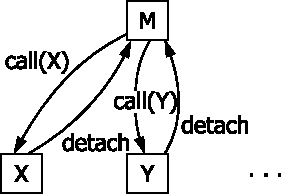
\includegraphics[width=\textwidth]{chap2/fig1}
	\caption{Representation of date (7, March, 1908)}
\end{figure}

A second occasion for using packed representations is when data storage is scarce, either in main store or on external backing stores. However, care must be taken that space saved on data storage is not outweighed by the expansion of the code which results from having to unpack and repack the data whenever it is inspected or updated.

The minimal representation is not often used for data storage, since the small amount of extra space it saves (always less than one bit per component) is usually more than outweighed by the extra time taken by multiplying and dividing on every access to the components, as compared with the more usual shifting and masking. However, the technique can be useful, possibly in conjunction with more conventional packing, if there is no other way of fitting the value within convenient word boundaries. Also, if the value is to be used solely or primarily as an index to a multi-dimensional array, the minimal representation is to be preferred; since this will save a significant amount of space in the representation of the array (see Section 6.2).

In representing the \textbf{with} construction in machine code, it is sometimes convenient to compute the address of the structure being referenced and store it in a register; this may achieve shorter and faster code for accessing the components. If the components have been packed, it may pay to unpack them into separate words before starting to process them, so that they can be easily referenced or updated; and if they have been updated, they must be packed up again and stored in the structure when the processing is complete. On some machines, it is more economic to pack and unpack a whole structure at the same time, rather than to perform these operations one at a time on the components.

\noindent
\textit{Exercise}

\noindent
Given a variable

\quad today:date;

\noindent
write a program to assign the value of the next following date to the variable tomorrow: date. Translate this program into the machine code of your choice using a tightly packed representation. Rewrite the program using an unpacked and then a minimal representation. Compare the lengths of the code involved, and the time taken to execute them.

\section{The discriminated union}

In defining sets of objects, it is often useful to define one set as the union of two previously known sets. For example, when jokers are added to a standard pack of cards, the extended set may be described as the union of the standard set plus the set consisting of the ``wild'' cards, joker I and joker 2. A type whose values range over the members of this set may be declared as the union of two alternatives, the card type, and an enumeration type with two distinct values:

\quad \textbf{type} pokercard $=$ (normal:($s$:suit; $r$:rank),

\tabto{10.2em}wild:(joker I, joker 2)).

\noindent
Each value of type pokercard corresponds either to an ordered pair with components indicating suit and rank; or else it corresponds to one of the two jokers in the enumeration type.

In specifying a constant of a discriminated union type, it is necessary to indicate to which of the alternative types the value denoted is intended to belong. This is done by writing the name of the alternative explicitly, for example:

\quad pokercard(normal(heart, Jack))

\noindent
denotes a value from the first alternative, whereas

\quad pokercard(wild(joker 2))

\noindent
denotes a value from the second alternative. In general, it is convenient to omit the type name, where the type can be inferred from context.

A second example of a discriminated union might be found in the maintenance of a register of all cars in a country. Cars may be distinguished as local cars owned by residents of the country, and visitor cars brought into the country temporarily by non-residents. The information required is rather different in the two cases. In both cases the number and the make of the car is considered relevant. However, for a local car, the name of the owner of the car is required, and the date on which the car was first registered in that owner's name. For visitor cars, this information is not relevant: all that is required is the standard three-letter abbreviation of the name of the country of origin. Thus the definition of the two alternative types of car might be:

\quad \textbf{type} local car = (make:manufacturer; regnumber:carnumber;

\tabto{9.4em} owner:person; first registration:date);

\quad \textbf{type} visitor car = (make:manufacturer; regnumber:carnumber;

\tabto{10.1em} origin:country);

Now it is possible to define a type covering both kinds of car:

\quad \textbf{type} car $=$ (local:local car,

\tabto{7.4em} foreign:visitor car).

\noindent
But here it is inconvenient to define the structure of local and foreign cars separately; and we would like to take advantage of the fact that several of their components are the same. This may be done by bringing the common components in front of both alternatives:

\quad \textbf{type} car $=$ (make:manufacturer;

\tabto{7.5em}regnumber:carnumber;

\tabto{7.5em}(local: (owner:person;

\tabto{7.8em}first registration:date),

\tabto{7.8em}foreign: (origin:country))

\tabto{7.1em}).

\noindent
Every car has a make and regnumber but only local cars have an owner or first registration date; and only foreign cars have an origin. 

A third example is the definition of geometric figures, which in some application might be categorized as either rectangles, triangles, or circles

\quad \textbf{type} figure $=$ (position:point; rect:$R$, tri:$T$, circ:$C$).

\noindent
The method of specifying the figure varies in each case. For a rectangle, the angle of inclination of one of the sides is given, together with the two lengths of the sides:

\quad \textbf{type} $R =$ (inclination:angle; side1, side2: real).

\noindent
A triangle is specified by the angle of inclination and length of one of its sides together with the angles formed between it and the other two sides:

\quad \textbf{type} $T =$ (inclination:angle; side:real; angle1, angle2:angle).

\noindent
For a circle, all that is necessary is to specify the diameter as a real number.

\quad \textbf{type} C $=$ (diameter:real).

When a type is defined as the union of several other types, it is important to recognize that its values must be considered wholly distinct from those of any of the types in terms of which it is defined. Otherwise there would be an immediate violation of the rule that each value belongs to only one type. Thus the union of types must be clearly distinguished from the normal concept of set union. Furthermore, for each element of the union type, it is possible to determine from which of the constituent types it originated, even if the same type has been repeated several times. For example, a double pack of cards used for playing patience may be defined as the union of two packs, i.e.,

\quad \textbf{type} patience card $=$ (red:cardface, blue:cardface).

\noindent
Each value of type patience card is clearly marked as having originated either from the red pack or from the blue pack, even if perhaps in the real world the colors of the backs are the same. This fact explains the use of the term ``discriminated union'' to apply to this form of type definition. It follows that the cardinality of a discriminated union is always the sum of the cardinalities of its constituent types.

\subsection{Manipulation}

Any value of a discriminated union carries with it a \textit{tag} field indicating which of the particular constituent types it originated from; on assignment this is copied, and on a test of equality, the tag fields must be the same if the values are to be equal.

Page 112

